\begin{frame}
	\frametitle{Outline}
	\begin{block}{Graph-based Approach}
		\begin{itemize}
			\item Transductive learning
			\item Present data on Graph
			\item Look for the separation between classes
			\item What happen if the separation is overlapped?
		\end{itemize}
	\end{block}
\end{frame}

\begin{frame}[fragile] 
	\frametitle{Graph Construction}
	\begin{figure}
		\begin{tikzpicture}
		\node[note](g) {$G=(V, E, W)$};
		\node[hightlight note, below of=g, xshift=-1.2cm](v) {Vertices $\{V_L, V_U\}$};
		\node[hightlight note, right of=v, xshift=1.1cm](e) {Edges};
		\node[hightlight note, right of=e, xshift=1.1cm](w) {Similarity weights};
		
		\draw[indicate arrow] (v) -- (g);
		\draw[indicate arrow] (e) -- ([xshift=.35cm]g.south);
		\draw[indicate arrow] (w) -- ([xshift=.85cm]g.south);
		\end{tikzpicture}
	\end{figure}
	
	\begin{figure}
		\begin{tikzpicture}[
		pics/randomgraph/.style = {
			code ={%
				\setcounter{c}{0};
				%
				\foreach \i/\j in {0/-.5,0/.5,2/-.5,2/.5}
				{
					\addtocounter{c}{1};
					\node[vertex](\thec) at (\i , \j){};
				}
				%
				\addtocounter{c}{1};
				\node[positive vertex, draw=none](\thec) at (1, 1.5){$+$};
				\addtocounter{c}{1};
				\node[negative vertex, draw=none](\thec) at (1, -1.5){$-$};
			}
		}]
		\node[node text, minimum width=50pt, minimum height=40pt](unlabel) at (0,0){Unlabeled};			
		\node[node text, minimum width=50pt, minimum height=17pt, above of=unlabel](label) {Labeled};
		\node[node text, below of=unlabel, draw=none]{Data set};
		
		\node[draw=none, right of=unlabel, yshift=.3cm, xshift=.6cm](arrow1) {$\rightarrow$};
		\node[node text, draw=none, above of=arrow1, yshift=-.65cm] {map}; 
		
		\pic[scale=1, right of=arrow1] {randomgraph};
		\foreach \i in {1,...,\thec}
		\foreach \j in {1,...,\thec}
		{
			\draw (\i) -- (\j);
		}
		
		\node[draw=none, right of=arrow1, xshift=3.cm](arrow2) {$\rightarrow$};
		\node[node text, draw=none, above of=arrow2, yshift=-.6cm] {sparsify}; 
		
		\pic[scale=1, right of=arrow2] {randomgraph};
		\foreach \i/\j in {5/2,5/4,2/4,6/1,6/3,1/3,1/2,3/4,6/2,5/3}
		{
			\draw (\i) -- (\j);
		}
		\end{tikzpicture}
	\end{figure}
	
	\pause
	\begin{block}{Some simple schedules}
		\begin{itemize}
			\item K most similar vertices for each vertex (kNN)
			\item Spanning tree with maximum weight (MST)
		\end{itemize}
	\end{block}
\end{frame}

\begin{frame}[fragile] 
	\frametitle{Sparse Graph Separation Assumption}
	\vspace{-1.3cm}
	\begin{figure}
		\centering
		\begin{tikzpicture}[
		scale=.7
		]
		\node[scale=.23](i) at (-.5,7) {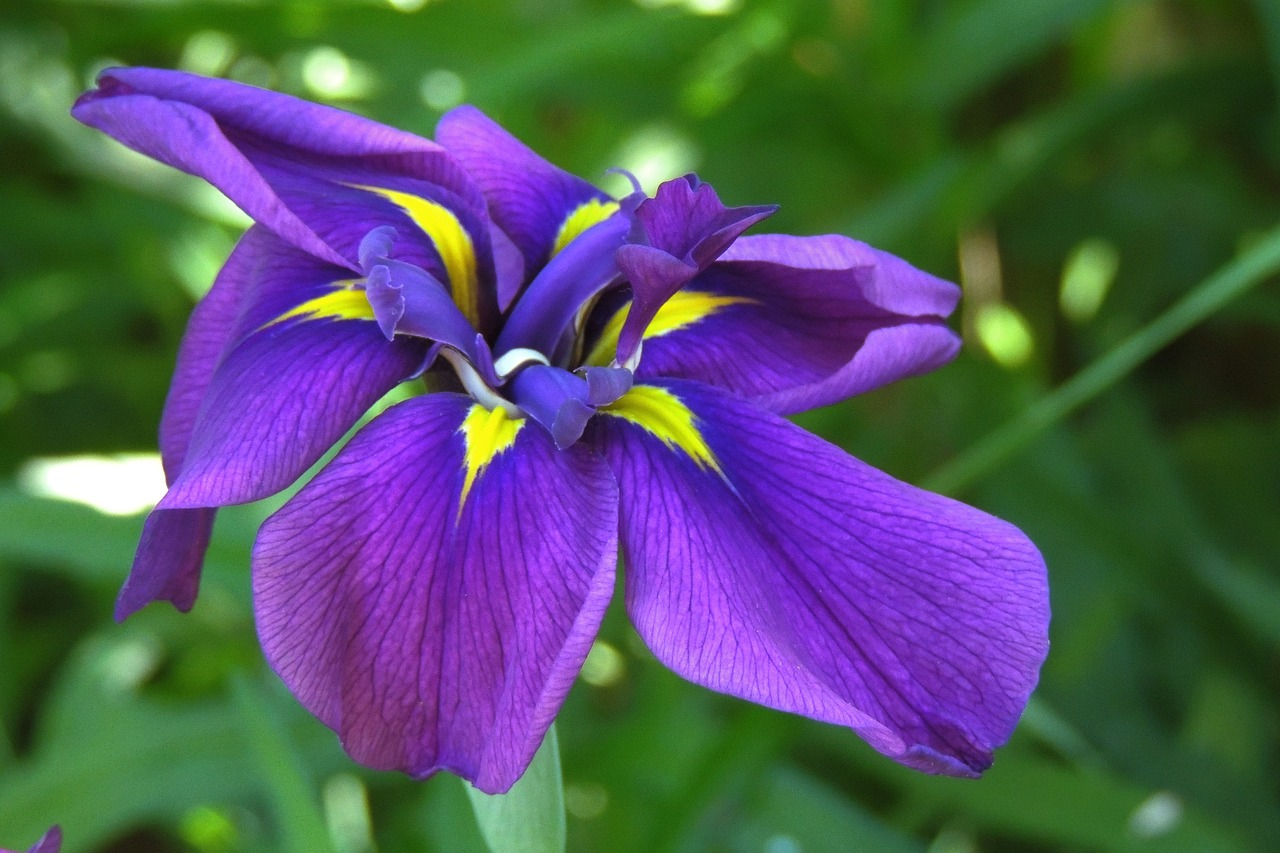
\includegraphics{data/iris.jpg}};
		\node[below of = i, yshift=-.35cm, node text, draw=none] {Iris data \\(150 instances, 4 features)};
		\coordinate(ii) at ($(i.center) + (5.5,0)$);
		\draw[thick, ->] ([xshift=3.5cm]i.center) -- (ii.center) 
		node[node text, above, midway, draw=none, yshift=.1cm]{kNN construction}
		node[node text, below, midway, draw=none, yshift=-.1cm]{(k=10)};
		\begin{axis}[
		hide x axis,
		hide y axis,
		xshift=3.5cm,
		yshift=2cm,
		scale=1.5
		]
		\addplot+[
		scatter,scatter src=explicit symbolic,
		draw=black,
		scatter/classes={
			1={mark=triangle,red},
			2={mark=o,blue}
		}] table[x=x,y=y,meta=class]{data/iris1.data};
		\addplot+[
		scatter,scatter src=explicit symbolic,
		draw=black,
		scatter/classes={
			0={mark=square,orange}
		}] table[x=x,y=y,meta=class]{data/iris2.data};
		% bound
		\addplot+[thick, cyan, smooth, mark=none] coordinates {(4.4,  1.9) (4.9,  1.65) (5.2, 1.65) (5.3,  1.5) (5.4,  1.2)};
		\addplot[thick, cyan, mark=none] coordinates { (2,1) (3,.5) };
		\node[hightlight note](l) at (axis cs:5,0.5){\large Separation boundary};
		\draw[indicate arrow] (l) -- (axis cs: 3.1, .5);
		\draw[indicate arrow] (l) -- (axis cs: 5.4, 1.1);
		\end{axis}
		\end{tikzpicture}
	\end{figure}
	
	\pause
	\vspace{-1.3cm}
	\begin{block}{Objective function}
		\vspace{-.5cm}
		\begin{align*}
		\argmin_{f} \quad \frac{1}{2}\sum_{(i,j) \in E}{W_{i,j}|f(i) - f(j)|}
		\end{align*}
		where $f(i) \in \{-1, +1\}$ represents label for $i \in V$.
	\end{block}
\end{frame}

\begin{frame}
	\frametitle{Minimum Cut Separation}
	\citeauthor{Blum:2001:LLU:645530.757779} in \citetitle{Blum:2001:LLU:645530.757779} gives a solution with a minimum cut on $G$
	\begin{figure}[!ht]
		\centering
		\captionsetup[subfigure]{justification=centering}
		\begin{subfigure}[b]{0.4\textwidth}
			\centering
			\begin{tikzpicture}[scale=1, auto,swap]
			% First we draw the vertices
			\foreach \pos/\label/\name in {
				{(0,0)/a/+}, {(1,0)/b/}, {(2,0)/c/},
				{(0,1)/e/+}, {(1,1)/f/}, {(2,1)/g/}}
			\node[positive vertex] (\label) at \pos{$\name$};
			
			\foreach \pos/\label/\name in {{(3,0)/d/-}, {(3,1)/h/-}}
			\node[negative vertex] (\label) at \pos{$\name$};
			
			% Connect vertices with edges and draw weights
			\foreach \source/ \dest in {
				b/e,b/g,d/g}
			\path[thickedge] (\source) -- (\dest);
			\foreach \source/ \dest in {
				a/b,a/e,b/c,c/d,d/h,e/f,f/g,g/h}
			\path[edge] (\source) -- (\dest);
			\end{tikzpicture}
			\caption*{Input graph $G$\\ \hfill }
		\end{subfigure}
		\hfill
		\begin{subfigure}[b]{0.5\textwidth}
			\centering
			\begin{tikzpicture}[scale=1, auto,swap]
			% First we draw the vertices
			\foreach \pos/\label/\name in {
				{(0,0)/a/+}, {(1,0)/b/}, {(2,0)/c/},
				{(0,1)/e/+}, {(1,1)/f/}, {(2,1)/g/}, {(-1,0.5)/v+/v_+}}
			\node[positive vertex] (\label) at \pos{$\name$};
			
			\foreach \pos/\label/\name in {{(3,0)/d/-}, {(3,1)/h/-}, {(4,0.5)/v-/v_-}}
			\node[negative vertex] (\label) at \pos{$\name$};
			
			% Connect vertices with edges and draw weights
			\foreach \source/ \dest in {
				b/e,b/g,d/g}
			\path[thickedge] (\source) -- (\dest);
			\foreach \source/ \dest in {
				a/b,a/e,b/c,c/d,d/h,e/f,f/g,g/h}
			\path[edge] (\source) -- (\dest);
			
			% inf weight
			\path[draw, line width=3pt] (v+) -- node[sloped, above]{\footnotesize $\infty$} (e);
			\path[draw, line width=3pt] (v-) -- node[sloped, above]{\footnotesize $\infty$} (h);
			
			\path[draw, line width=3pt] (v+) -- node[sloped, below]{\footnotesize $\infty$} (a);
			\path[draw, line width=3pt] (v-) -- node[sloped, below]{\footnotesize $\infty$} (d);
			\end{tikzpicture}
			\caption*{Step 1, add pseudo vertices $v_+, v_-$ and corresponding edges}
		\end{subfigure}
		
		\pause
		\vspace*{5pt}
		\begin{subfigure}[b]{0.5\textwidth}
			\centering
			\begin{tikzpicture}[scale=1, auto,swap]
			% First we draw the vertices
			\foreach \pos/\label/\name in {
				{(0,0)/a/+}, {(1,0)/b/}, {(2,0)/c/},
				{(0,1)/e/+}, {(1,1)/f/}, {(2,1)/g/}, {(-1,0.5)/v+/v_+}}
			\node[positive vertex] (\label) at \pos{$\name$};
			
			\foreach \pos/\label/\name in {{(3,0)/d/-}, {(3,1)/h/-}, {(4,0.5)/v-/v_-}}
			\node[negative vertex] (\label) at \pos{$\name$};
			
			% Connect vertices with edges and draw weights
			\foreach \source/ \dest in {
				b/e,b/g,d/g}
			\path[thickedge] (\source) -- (\dest);
			\foreach \source/ \dest in {
				a/b,a/e,b/c,c/d,d/h,e/f,f/g,g/h}
			\path[edge] (\source) -- (\dest);
			
			% inf weight
			\path[draw, line width=3pt] (v+) -- node[sloped, above]{\footnotesize $\infty$} (e);
			\path[draw, line width=3pt] (v-) -- node[sloped, above]{\footnotesize $\infty$} (h);
			
			\path[draw, line width=3pt] (v+) -- node[sloped, below]{\footnotesize $\infty$} (a);
			\path[draw, line width=3pt] (v-) -- node[sloped, below]{\footnotesize $\infty$} (d);
			
			\path[dashedge] (1.5, 1.5) -- (1.5, -0.5);
			\end{tikzpicture}
			\caption*{Step 2, find a minimum cut in G with source $v_+$ and sink $v_-$}
		\end{subfigure}
		\hfill
		\begin{subfigure}[b]{0.4\textwidth}
			\centering
			\begin{tikzpicture}[scale=1, auto,swap]
			% First we draw the vertices
			% First we draw the vertices
			\foreach \pos/\label/\name in {
				{(0,0)/a/+}, {(0,1)/e/+}, {(1,0)/b/+}, {(1,1)/f/+}}
			\node[positive vertex] (\label) at \pos{$\name$};
			
			\foreach \pos/\label/\name in {
				{(3,0)/d/-}, {(3,1)/h/-}, {(2,1)/g/-}, {(2,0)/c/-}}
			\node[negative vertex] (\label) at \pos{$\name$};
			
			% Connect vertices with edges and draw weights
			\foreach \source/ \dest in {
				b/e,b/g,d/g}
			\path[thickedge] (\source) -- (\dest);
			\foreach \source/ \dest in {
				a/b,a/e,b/c,c/d,d/h,e/f,f/g,g/h}
			\path[edge] (\source) -- (\dest);
			
			\path[dashedge] (1.5, 1.5) -- (1.5, -0.5);
			\end{tikzpicture}
			\caption*{Step 3, use this cut to label unlabeled vertices}
		\end{subfigure}
	\end{figure}
\end{frame}

\begin{frame}
	\frametitle{When the Boundary Is Collapsed}
	A graph may have more than one positive solution and can cause the degenerate inference.
	\begin{figure}
		\centering
		\begin{tikzpicture}[scale=1.3, auto,swap]
		% First we draw the vertices
		\foreach \pos/\label/\name in {
			{(0,0)/a/+}, {(1,0)/b/}, {(2,0)/c/}, {(3,0)/d/}, {(4,0)/e/},
			{(0,1)/g/+}, {(1,1)/h/}, {(2,1)/i/}, {(3,1)/j/}, {(4,1)/k/}}
		\node[positive vertex] (\label) at \pos{$\name$};
		
		\foreach \pos/\label/\name in {{(5,0)/f/-}, {(5,1)/l/-}}
		\node[negative vertex] (\label) at \pos{$\name$};
		
		\foreach \pos/\label in {{(2.5, 0)/x1}, {(2.5, 1)/x2}}
		\node (\label) at \pos{$\dots$};
		
		% Connect vertices with edges and draw weights
		\foreach \source/ \dest in {
			a/h, h/c, j/e, e/l}
		\path[thickedge] (\source) -- (\dest);
		\foreach \source/ \dest in {
			a/b, b/c, d/e, e/f, f/l, l/k, k/j, i/h, h/g, g/a}
		\path[edge] (\source) -- (\dest);
		
		\path[dashedge] (.5, 1.2) -- (.5, -0.2);
		\node[note] at (.5,1.5) {$C_1$};
		\path[dashedge] (1.5, 1.2) -- (1.5, -0.2);
		\path[dashedge] (3.5, 1.2) -- (3.5, -0.2);
		\path[dashedge] (4.5, 1.2) -- (4.5, -0.2);
		\node[note] at (4.5,1.5) {$C_2$};
		\end{tikzpicture}
	\end{figure}
	$\rightarrow$ The need for a balanced separation.
	
	\pause
	\begin{itemize}
		\item Loop for all positive separations and choose the best
		\item Add random noise to have better change of the right boundary (\textit{randomized mincut}, \citeauthor{Blum:2004:SLU:1015330.1015429})
		\item \textbf{Intervene the reasoning process}
	\end{itemize}
\end{frame}

\begin{frame}
	\frametitle{Graphical Model}
	Consider the vertices as random variables
	\begin{align*}
	X = \{X_i : i \in V, X_i = f(i) \}
	\end{align*}
	
	\pause
	We define a set of independent factors. Assume that the implied distribution of $X$ only depends on $\Phi$
	\begin{align*}
	\Phi = \{ \phi_{i,j} : (i,j) \in E, \phi_{i,j} = \exp(-W_{i,j}(X_i - X_j)^2) \}
	\end{align*}
	
	\begin{figure}
		\centering
		\begin{tikzpicture}
		\node[positive vertex](x1) at (0,0){};
		\node[node text, draw=none, below of=x1, yshift=.5cm]{$X_1$};
		\node[vertex, rectangle, right of=x1](p1){};
		\node[node text, draw=none, below of=p1, yshift=.5cm]{$\phi_{1,2}$};
		\node[positive vertex, right of=p1](x2){};
		\node[node text, draw=none, below of=x2, yshift=.5cm]{$X_2$};
		
		\node[vertex, draw=none, right of=x2](xd){$\dots$};
		
		\node[positive vertex, right of=xd](xn-1){};
		\node[node text, draw=none, below of=xn-1, yshift=.5cm]{$X_{n-1}$};
		\node[vertex, rectangle, right of=xn-1](pn){};
		\node[node text, draw=none, below of=pn, yshift=.5cm]{$\phi_{n-1,n}$};
		\node[positive vertex, right of=pn](xn){};
		\node[node text, draw=none, below of=xn, yshift=.5cm]{$X_{n}$};
		
		\draw (x1) -- (p1);
		\draw (p1) -- (x2);
		\draw (x2) -- (xd);
		\draw (xd) -- (xn-1);
		\draw (xn-1) -- (pn);
		\draw (pn) -- (xn);
		\end{tikzpicture}
	\end{figure}
	
	\pause
	We are looking for a configuration $X_{max}$ of $X$ that
	\begin{align*}
	P_\Phi(X_{max}) = \max_X{P_\Phi}
	\end{align*}
\end{frame}

\begin{frame}
	\frametitle{Influence Index}
	The inference can be represented in a message sending schedule
	
	\begin{columns}
		\column{.5\textwidth}
		\begin{figure}
			\centering
			\begin{tikzpicture}
			\node[positive vertex](x1) at (0,0){};
			\node[node text, left of=x1, draw=none, xshift=.6cm]{$X_1$};
			\node[positive vertex, right of=x1, xshift=.5cm](x2){};
			\node[node text, left of=x2, draw=none, xshift=.6cm]{$X_2$};
			\node[positive vertex, above of=x1, yshift=.5cm](x3){};
			\node[node text, left of=x3, draw=none, xshift=.6cm]{$X_3$};
			\node[positive vertex, right of=x3, xshift=.5cm](x4){};
			\node[node text, left of=x4, draw=none, xshift=.6cm]{$X_4$};
			\node[positive vertex, above of=x3, yshift=.5cm](x5){};
			\node[node text, left of=x5, draw=none, xshift=.6cm]{$X_5$};
			
			\draw[->] (x1)--(x3) node[left, midway, node text, draw=none, blue]{$\psi_{X_1,X_3}$};
			\draw[->] (x2)--(x3) node[right, midway, node text, draw=none, blue, xshift=.1cm]{$\psi_{X_2,X_3}$};
			\draw[->] (x3)--(x5) node[left, midway, node text, draw=none, blue]{$\psi_{X_3,X_5}$};
			\draw[->] (x4)--(x5) node[right, midway, node text, draw=none, blue, xshift=.1cm]{$\psi_{X_4,X_5}$};
			
			\node[hightlight note, below right of = x2, xshift=.5cm](leaf){Leaf};
			\draw[indicate arrow](leaf)--(x1.south);
			\draw[indicate arrow](leaf)--(x2);
			\draw[indicate arrow](leaf)--(x4);
			
			\node[hightlight note, right of = x5, xshift=.5cm](root){Root};
			\draw[indicate arrow](root)--(x5);
			\end{tikzpicture}
		\end{figure}
	
		\pause
		\column{.5\textwidth}
		\begin{figure}
			\centering
			\begin{tikzpicture}
			% First we draw the vertices
			\foreach \pos/\label in {
				{(0,0)/a}, {(0,1)/b}}
			\node[positive vertex] (\label) at \pos{};
			\node at (0,0.56){$\vdots$};
			
			\node[dashed, draw, ellipse, 
			minimum height=1.8cm, minimum width=.7cm,
			label=above:{$\scriptstyle ne(i)/j$}] at (0,0.5) {};
			
			\foreach \pos/\label/\name in {
				{(1,0.5)/i/X_i}, {(2,0.5)/j/X_j}}
			\node[positive vertex, label={$\name$}] (\label) at \pos{};
			
			\foreach \source/ \dest in {
				a/i, b/i, i/j}
			\path[edge, ->] (\source) -- (\dest);
			\end{tikzpicture}
		\end{figure}
		
		More possible solutions with equal condition
		\begin{align*}
		\psi_{-1, X_j} = \psi_{+1, X_j}
		\end{align*}
	\end{columns}
	
	\pause
	\vspace{.5cm}
	\textcolor{blue}{We can replace it with the Influence index}
	\begin{align*}
	\textnormal{influence}_{i \in V_U} = \argmax_{X_i}{ \sum_{X_i = X_j, \forall j \in V_L}{W_{i, j}} }
	\end{align*}
\end{frame}

\begin{frame}
	\frametitle{Loopy Belief Propagation Algorithm}
	Message sending is not guaranteed when we have circles in $G$\\
	\pause
	\vspace{.5cm}
	\begin{columns}
		\column{.3\textwidth}
		\vspace{-.5cm}
		\begin{figure}
			\centering
			\begin{tikzpicture}
			\node[positive vertex](x1) at (0,0){};
			\node[node text, left of=x1, draw=none, xshift=.6cm]{$X_1$};
			\node[positive vertex, right of=x1, xshift=.5cm](x2){};
			\node[node text, right of=x2, draw=none, xshift=-.6cm]{$X_2$};
			\node[positive vertex, above of=x1, yshift=.5cm](x3){};
			\node[node text, left of=x3, draw=none, xshift=.6cm]{$X_3$};
			\node[positive vertex, right of=x3, xshift=.5cm](x4){};
			\node[node text, right of=x4, draw=none, xshift=-.6cm]{$X_4$};
			\node[positive vertex, above of=x3, yshift=.5cm](x5){};
			\node[node text, left of=x5, draw=none, xshift=.6cm]{$X_5$};
			
			\draw[<->] (x1)--(x3) node[left, midway, node text, draw=none, blue]{$\psi_{X_1,X_3}$\\$\psi_{X_3,X_1}$};
			\draw[<->] (x2)--(x3) node[right, pos=.7, node text, draw=none, blue, xshift=.3cm]{$\psi_{X_2,X_3}$\\$\psi_{X_3,X_2}$};
			\draw[<->] (x3)--(x5) node[left, midway, node text, draw=none, blue]{$\psi_{X_3,X_5}$\\$\psi_{X_5,X_3}$};
			\draw[<->] (x4)--(x5) node[right, pos=.7, node text, draw=none, blue, xshift=.3cm]{$\psi_{X_4,X_5}$\\$\psi_{X_5,X_4}$};
			\draw[<->] (x1)--(x2) node[below, midway, node text, draw=none, blue]{$\psi_{X_1,X_2}$\\$\psi_{X_2,X_1}$};
			\end{tikzpicture}
		\end{figure}
		\column{.7\textwidth}
		The approximate loopy process
		\begin{itemize}
			\item Messages will be sent from both directions, all at the same time.
			\item The decision will be made on all neighbor vertices
			$P_\Phi(X_i) = \underset{X_i}{\max{}} \prod_{k\in ne(i)} \psi_{X_k, X_i}$
		\end{itemize}
	\end{columns}
	
	\pause
	\vspace{.3cm}
	$\rightarrow$ We can only check the equal condition (when using influence index) after the loop is finished
	\begin{align*}
	\prod_{k\in ne(i)} \psi_{X_k, -1} = \prod_{k\in ne(i)} \psi_{X_k, +1}
	\end{align*}
\end{frame}

\begin{frame}
	\frametitle{Synthetic Data}
	\vspace{-.2cm}
	\begin{figure}
		\centering
		\begin{subfigure}[b]{0.31\textwidth}
			\centering
			\begin{tikzpicture}[scale=.5]
			\begin{tikzpicture}[scale=.95, auto,swap]\tiny
% First we draw the vertices

\foreach \pos/\label/\name in {
	{(-0.2225200774229265,-0.32608517245672425)/0/-},
	{(-0.10792698973224357,-0.4322723564304132)/1/-},
	{(-0.43579819547117127,-0.2585310210445544)/2/-},
	{(-0.5098276643544934,-0.06199801779890762)/3/-},
	{(-0.3572219112967324,-0.2901705254124338)/4/-},
	{(-0.24686014357506988,-0.26602094982298574)/5/-},
	{(-0.4122781181743554,-0.41174037627413024)/6/-},
	{(-0.13155402521469958,-0.28265284939268)/7/-},
	{(-0.4013892200821219,0.6194130925380561)/8/-},
	{(-0.038682149507085886,-0.8841269464236071)/9/-},
	{(0.41775279311705266,0.5452836919306788)/10/-},
	{(1.1904429279543804,0.12934373248317083)/11/-},
	{(-0.41432691418775425,0.5020246503499929)/12/-},
	{(-0.14889652692904784,0.1881127108599629)/13/-},
	{(0.9065568090920573,-0.04785238879610198)/14/-},
	{(-0.7610715120240329,0.272872387134225)/15/-},
	{(-0.861744815921591,-0.7708778060573379)/16/-},
	{(1.2616790328054561,0.47283622148673293)/17/-},
	{(0.8823972087062629,0.6771687409090151)/18/-},
	{(0.907386175227952,0.10201909787511977)/19/-},
	{(0.8151941545969827,-1.3229401390732802)/20/-},
	{(-0.3600809460549404,0.11375713002443522)/21/-},
	{(-0.6216368891606755,-0.011828622788958848)/22/-},
	{(0.3886482458977085,0.28519842097236453)/23/-},
	{(0.3739640144981814,0.24875347122026437)/24/-},
	{(-0.7003448143329841,0.12648214505188243)/25/-},
	{(1.1228951823756235,0.03345266618831543)/26/-},
	{(-0.5514053331935688,0.3486980144610941)/27/-},
	{(-0.8405414751795116,0.1008419612116009)/28/-},
	{(-0.22755600921330738,0.5053911984153584)/29/-},
	{(1.2312831692458468,-0.48487307878717706)/30/-},
	{(-0.14880270817774913,-0.004411244360598876)/31/-},
	{(-1.0214210116630718,-0.7200578453405849)/32/-},
	{(-1.682542920343154,0.8120634506562726)/33/-},
	{(0.5197389699875548,0.05911408349384489)/34/-},
	{(0.20624066023889748,-0.6735203793700854)/35/-},
	{(0.2625139378422709,0.1015979089411237)/36/-},
	{(0.8656010941779964,1.059276248934198)/37/-},
	{(0.2826750077050263,-0.07536302179574172)/38/-},
	{(-0.03852398821741344,-0.48227286214472553)/39/-},
	{(-0.28136151536478954,-0.39446624795812957)/40/-},
	{(-0.3313024644512042,0.02157567131174938)/41/-},
	{(0.6100935009885826,-0.6508235109140897)/42/-},
	{(0.052363422936958025,-0.8095424543799895)/43/-},
	{(0.9489381699005437,0.022268071023513282)/44/-},
	{(0.7672476712214347,0.9844728333954431)/45/-},
	{(-0.22182434386182312,0.27963221298609403)/46/-},
	{(0.7766120290084281,-0.2711325015401132)/47/-},
	{(1.0496911867665026,0.5156493304744518)/48/-},
	{(0.8127325614994425,0.16476250666194273)/49/-},
	{(0.2642720963285284,-1.0959841681624427)/50/-},
	{(-1.3666758090695248,-0.00713893417170424)/51/-},
	{(-0.3650145326840327,-0.6730504611209082)/52/-},
	{(-0.3963669255792561,0.5608056869929939)/53/-},
	{(-0.11636929333258177,0.2391172613141169)/54/-},
	{(0.6136753954272933,-0.1613504080046083)/55/-},
	{(-0.0672994614932272,-0.7602379191233869)/56/-},
	{(0.6844367301222299,-0.9740555320476774)/57/-},
	{(0.440420203987672,-0.027778616760857164)/58/-},
	{(0.35719629151702703,-0.30007006274736503)/59/-},
	{(-1.2309475650684873,0.6790650053498698)/60/-},
	{(-0.5994086559093385,0.07646944266252349)/61/-},
	{(0.6197286517310527,-0.11730351058171999)/62/-},
	{(0.21958763515861823,0.10611875050675876)/63/-},
	{(-0.5883992127404697,-0.8308609217808781)/64/-},
	{(-0.3369916105527138,0.7856073817078143)/65/-},
	{(0.5590809097148529,0.26175750577408813)/66/-},
	{(0.4250671397900095,-0.26710133363366423)/67/-},
	{(-0.7875100948809406,1.1398016134428481)/68/-},
	{(0.8521281146228749,0.35319582635900426)/69/-},
	{(0.18895715421089304,-0.5528070760114767)/70/-},
	{(-0.21374246039691278,-0.6394027771092863)/71/-},
	{(1.608251500873829,-0.11895206781670753)/72/-},
	{(0.1722636294332391,0.2207040736771844)/73/-},
	{(-0.10617942514952022,0.6069284647949044)/74/-},
	{(0.2676644060568022,-0.49789415396759906)/75/-}}
\node[negative vertex,synthetic data, draw=none] (\label) at \pos{$\pmb{\name}$};

\foreach \pos/\label/\name in {
	{(1.2326160752073525,1.3234376541212238)/0/+},
	{(1.18126634100516,1.409284058060322)/1/+},
	{(1.283707993678125,1.4311581195421956)/2/+},
	{(1.3989139742981929,1.566047516510241)/3/+},
	{(1.0407760297608515,1.5419064995316616)/4/+},
	{(1.21253590460229,1.2910005600863865)/5/+},
	{(1.2020405154165823,1.40420139366607)/6/+},
	{(1.2392101116906649,1.488783260262376)/7/+},
	{(1.1468176063819597,0.21654487509179432)/8/+},
	{(1.5312777468623744,1.8240008183654495)/9/+},
	{(0.17436518741550844,0.8372839224318885)/10/+},
	{(1.2280673693945807,1.9201724818731143)/11/+},
	{(1.8757259915151439,-0.04678741181443402)/12/+},
	{(-0.167057321969035,0.9789254048224365)/13/+},
	{(0.4304282060887261,0.21051634303401157)/14/+},
	{(1.5753243355301219,0.31572908830356494)/15/+},
	{(1.2445627087126905,0.8831764393154039)/16/+},
	{(1.686471444435738,1.355538138968294)/17/+},
	{(0.9130990594940642,0.8022306819824563)/18/+},
	{(1.6182585102411458,2.0218370328165887)/19/+},
	{(1.9073967440451707,1.6256427879170825)/20/+},
	{(0.22772542588568312,2.2534260011202747)/21/+},
	{(1.733546091697963,1.8984075277942165)/22/+},
	{(0.086893309837621,1.1006261376533484)/23/+},
	{(1.1193119918417844,1.4751070236904238)/24/+},
	{(1.5330537588631583,0.6433292500778514)/25/+},
	{(1.2187062333932948,1.106573406164404)/26/+},
	{(0.37585370102897564,1.4768547457515944)/27/+},
	{(0.5822539624502868,0.9641504363279036)/28/+},
	{(0.5919393941374593,0.9611956521082146)/29/+},
	{(1.0331207611246993,1.0647265591083686)/30/+},
	{(0.9231900767872212,0.6267526504907435)/31/+},
	{(1.8909620118270127,0.718533865252585)/32/+},
	{(0.44507402088776205,0.27094705049763224)/33/+},
	{(1.1164361204277515,0.8765220720175932)/34/+},
	{(1.188133860698395,1.3357523587585303)/35/+},
	{(1.243834254590601,0.8436510348972432)/36/+},
	{(0.7541845778436342,1.9197879281891508)/37/+},
	{(1.0924819941877562,0.5614407575650796)/38/+},
	{(-0.5112210572032863,1.2035737602595757)/39/+},
	{(0.9354912248232083,0.9998490458933262)/40/+},
	{(0.5148907067181836,1.553098215588476)/41/+},
	{(0.22289394571229248,0.9300685317992426)/42/+},
	{(0.45146645247925943,2.6395987932987923)/43/+},
	{(-0.166424060712552,1.3706437709167607)/44/+},
	{(1.1614859876291066,1.0139615483688815)/45/+},
	{(0.2315193712234055,1.0575460834275956)/46/+},
	{(1.3376857163351328,1.4701544761758611)/47/+},
	{(1.9990885932355438,1.598302649463204)/48/+},
	{(0.23366253082156352,1.3289488752291043)/49/+},
	{(1.184440118690655,0.3220342344237722)/50/+},
	{(1.6629785147905967,0.2791844298487036)/51/+},
	{(-0.2392090208428923,0.9283570167288818)/52/+},
	{(0.3294869991553525,-0.1340161763586405)/53/+},
	{(2.157308879298305,1.2301984256501093)/54/+},
	{(0.8890881019229913,1.3825220366540856)/55/+},
	{(-0.3070953393572853,1.1771520885350466)/56/+},
	{(1.4201643493322353,0.860774669113443)/57/+},
	{(1.241098553848087,1.1802593196970175)/58/+},
	{(0.05191678988226933,1.3335726259621392)/59/+},
	{(0.875423132354217,0.41366037925611177)/60/+},
	{(0.8508546465756415,0.40358639942872676)/61/+},
	{(1.9197719023285993,2.7009744997622187)/62/+},
	{(1.1215047479185833,0.912333711433073)/63/+},
	{(0.6025422400785359,0.9841423427079677)/64/+},
	{(-0.1085417345449402,0.331130854509775)/65/+},
	{(2.2059440168255167,0.3782987337349223)/66/+},
	{(1.1678102698129817,1.1043382891263502)/67/+},
	{(1.2485051805588707,0.5931143672895391)/68/+},
	{(1.1791800893144846,0.28317729086784493)/69/+},
	{(-0.12423887021360702,0.6666205633386242)/70/+},
	{(1.5962315209365912,-0.10666504357026674)/71/+},
	{(1.64669426796325,0.7028638139972351)/72/+},
	{(1.8357330498023554,1.3102657969459173)/73/+},
	{(2.3772912710679828,0.8411082602923297)/74/+},
	{(0.5026524784873001,1.0069292252112034)/75/+}}
\node[positive vertex, synthetic data, draw=none] (\label) at \pos{$\pmb{\name}$};

%\draw [red] (0,0) circle [radius=0.6*1.96 ];
%\draw [blue] (1,1) circle [radius=0.6*1.96 ];

\end{tikzpicture}
			\end{tikzpicture}
			\caption{True data}
		\end{subfigure}
		\hfill
		\begin{subfigure}[b]{0.31\textwidth}
			\centering
			\begin{tikzpicture}[scale=.5]
			\begin{tikzpicture}[scale=.95, auto,swap]\tiny
% First we draw the vertices

\foreach \pos/\label/\name in {
	{(-0.2225200774229265,-0.32608517245672425)/0/-},
	{(-0.10792698973224357,-0.4322723564304132)/1/-},
	{(-0.43579819547117127,-0.2585310210445544)/2/-},
	{(-0.5098276643544934,-0.06199801779890762)/3/-},
	{(-0.3572219112967324,-0.2901705254124338)/4/-},
	{(-0.24686014357506988,-0.26602094982298574)/5/-},
	{(-0.4122781181743554,-0.41174037627413024)/6/-},
	{(-0.13155402521469958,-0.28265284939268)/7/-},
	{(-0.4013892200821219,0.6194130925380561)/8/-},
	{(-0.038682149507085886,-0.8841269464236071)/9/-},
	{(0.41775279311705266,0.5452836919306788)/10/-},
	{(-0.41432691418775425,0.5020246503499929)/11/-},
	{(-0.14889652692904784,0.1881127108599629)/12/-},
	{(0.9065568090920573,-0.04785238879610198)/13/-},
	{(-0.7610715120240329,0.272872387134225)/14/-},
	{(-0.861744815921591,-0.7708778060573379)/15/-},
	{(0.907386175227952,0.10201909787511977)/16/-},
	{(0.8151941545969827,-1.3229401390732802)/17/-},
	{(-0.3600809460549404,0.11375713002443522)/18/-},
	{(-0.6216368891606755,-0.011828622788958848)/19/-},
	{(0.3886482458977085,0.28519842097236453)/20/-},
	{(0.3739640144981814,0.24875347122026437)/21/-},
	{(-0.7003448143329841,0.12648214505188243)/22/-},
	{(-0.5514053331935688,0.3486980144610941)/23/-},
	{(-0.8405414751795116,0.1008419612116009)/24/-},
	{(-0.22755600921330738,0.5053911984153584)/25/-},
	{(-0.14880270817774913,-0.004411244360598876)/26/-},
	{(-1.0214210116630718,-0.7200578453405849)/27/-},
	{(-1.682542920343154,0.8120634506562726)/28/-},
	{(0.5197389699875548,0.05911408349384489)/29/-},
	{(0.20624066023889748,-0.6735203793700854)/30/-},
	{(0.2625139378422709,0.1015979089411237)/31/-},
	{(0.2826750077050263,-0.07536302179574172)/32/-},
	{(-0.03852398821741344,-0.48227286214472553)/33/-},
	{(-0.28136151536478954,-0.39446624795812957)/34/-},
	{(-0.3313024644512042,0.02157567131174938)/35/-},
	{(0.6100935009885826,-0.6508235109140897)/36/-},
	{(0.052363422936958025,-0.8095424543799895)/37/-},
	{(0.9489381699005437,0.022268071023513282)/38/-},
	{(-0.22182434386182312,0.27963221298609403)/39/-},
	{(0.7766120290084281,-0.2711325015401132)/40/-},
	{(0.8127325614994425,0.16476250666194273)/41/-},
	{(0.2642720963285284,-1.0959841681624427)/42/-},
	{(-1.3666758090695248,-0.00713893417170424)/43/-},
	{(-0.3650145326840327,-0.6730504611209082)/44/-},
	{(-0.3963669255792561,0.5608056869929939)/45/-},
	{(-0.11636929333258177,0.2391172613141169)/46/-},
	{(0.6136753954272933,-0.1613504080046083)/47/-},
	{(-0.0672994614932272,-0.7602379191233869)/48/-},
	{(0.6844367301222299,-0.9740555320476774)/49/-},
	{(0.440420203987672,-0.027778616760857164)/50/-},
	{(0.35719629151702703,-0.30007006274736503)/51/-},
	{(-1.2309475650684873,0.6790650053498698)/52/-},
	{(-0.5994086559093385,0.07646944266252349)/53/-},
	{(0.6197286517310527,-0.11730351058171999)/54/-},
	{(0.21958763515861823,0.10611875050675876)/55/-},
	{(-0.5883992127404697,-0.8308609217808781)/56/-},
	{(-0.3369916105527138,0.7856073817078143)/57/-},
	{(0.5590809097148529,0.26175750577408813)/58/-},
	{(0.4250671397900095,-0.26710133363366423)/59/-},
	{(-0.7875100948809406,1.1398016134428481)/60/-},
	{(0.18895715421089304,-0.5528070760114767)/61/-},
	{(-0.21374246039691278,-0.6394027771092863)/62/-},
	{(0.1722636294332391,0.2207040736771844)/63/-},
	{(-0.10617942514952022,0.6069284647949044)/64/-},
	{(0.2676644060568022,-0.49789415396759906)/65/-},
	{(-0.167057321969035,0.9789254048224365)/66/-},
	{(0.4304282060887261,0.21051634303401157)/67/-},
	{(0.44507402088776205,0.27094705049763224)/68/-},
	{(-0.5112210572032863,1.2035737602595757)/69/-},
	{(-0.2392090208428923,0.9283570167288818)/70/-},
	{(0.3294869991553525,-0.1340161763586405)/71/-},
	{(-0.3070953393572853,1.1771520885350466)/72/-},
	{(-0.1085417345449402,0.331130854509775)/73/-},
	{(-0.12423887021360702,0.6666205633386242)/74/-}}
	\node[negative vertex,synthetic data, draw=none] (\label) at \pos{$\pmb{\name}$};

\foreach \pos/\label/\name in {
	{(1.2326160752073525,1.3234376541212238)/0/+},
	{(1.18126634100516,1.409284058060322)/1/+},
	{(1.283707993678125,1.4311581195421956)/2/+},
	{(1.3989139742981929,1.566047516510241)/3/+},
	{(1.0407760297608515,1.5419064995316616)/4/+},
	{(1.21253590460229,1.2910005600863865)/5/+},
	{(1.2020405154165823,1.40420139366607)/6/+},
	{(1.2392101116906649,1.488783260262376)/7/+},
	{(1.1904429279543804,0.12934373248317083)/8/+},
	{(1.2616790328054561,0.47283622148673293)/9/+},
	{(0.8823972087062629,0.6771687409090151)/10/+},
	{(1.1228951823756235,0.03345266618831543)/11/+},
	{(1.2312831692458468,-0.48487307878717706)/12/+},
	{(0.8656010941779964,1.059276248934198)/13/+},
	{(0.7672476712214347,0.9844728333954431)/14/+},
	{(1.0496911867665026,0.5156493304744518)/15/+},
	{(0.8521281146228749,0.35319582635900426)/16/+},
	{(1.608251500873829,-0.11895206781670753)/17/+},
	{(1.1468176063819597,0.21654487509179432)/18/+},
	{(1.5312777468623744,1.8240008183654495)/19/+},
	{(0.17436518741550844,0.8372839224318885)/20/+},
	{(1.2280673693945807,1.9201724818731143)/21/+},
	{(1.8757259915151439,-0.04678741181443402)/22/+},
	{(1.5753243355301219,0.31572908830356494)/23/+},
	{(1.2445627087126905,0.8831764393154039)/24/+},
	{(1.686471444435738,1.355538138968294)/25/+},
	{(0.9130990594940642,0.8022306819824563)/26/+},
	{(1.6182585102411458,2.0218370328165887)/27/+},
	{(1.9073967440451707,1.6256427879170825)/28/+},
	{(0.22772542588568312,2.2534260011202747)/29/+},
	{(1.733546091697963,1.8984075277942165)/30/+},
	{(0.086893309837621,1.1006261376533484)/31/+},
	{(1.1193119918417844,1.4751070236904238)/32/+},
	{(1.5330537588631583,0.6433292500778514)/33/+},
	{(1.2187062333932948,1.106573406164404)/34/+},
	{(0.37585370102897564,1.4768547457515944)/35/+},
	{(0.5822539624502868,0.9641504363279036)/36/+},
	{(0.5919393941374593,0.9611956521082146)/37/+},
	{(1.0331207611246993,1.0647265591083686)/38/+},
	{(0.9231900767872212,0.6267526504907435)/39/+},
	{(1.8909620118270127,0.718533865252585)/40/+},
	{(1.1164361204277515,0.8765220720175932)/41/+},
	{(1.188133860698395,1.3357523587585303)/42/+},
	{(1.243834254590601,0.8436510348972432)/43/+},
	{(0.7541845778436342,1.9197879281891508)/44/+},
	{(1.0924819941877562,0.5614407575650796)/45/+},
	{(0.9354912248232083,0.9998490458933262)/46/+},
	{(0.5148907067181836,1.553098215588476)/47/+},
	{(0.22289394571229248,0.9300685317992426)/48/+},
	{(0.45146645247925943,2.6395987932987923)/49/+},
	{(-0.166424060712552,1.3706437709167607)/50/+},
	{(1.1614859876291066,1.0139615483688815)/51/+},
	{(0.2315193712234055,1.0575460834275956)/52/+},
	{(1.3376857163351328,1.4701544761758611)/53/+},
	{(1.9990885932355438,1.598302649463204)/54/+},
	{(0.23366253082156352,1.3289488752291043)/55/+},
	{(1.184440118690655,0.3220342344237722)/56/+},
	{(1.6629785147905967,0.2791844298487036)/57/+},
	{(2.157308879298305,1.2301984256501093)/58/+},
	{(0.8890881019229913,1.3825220366540856)/59/+},
	{(1.4201643493322353,0.860774669113443)/60/+},
	{(1.241098553848087,1.1802593196970175)/61/+},
	{(0.05191678988226933,1.3335726259621392)/62/+},
	{(0.875423132354217,0.41366037925611177)/63/+},
	{(0.8508546465756415,0.40358639942872676)/64/+},
	{(1.9197719023285993,2.7009744997622187)/65/+},
	{(1.1215047479185833,0.912333711433073)/66/+},
	{(0.6025422400785359,0.9841423427079677)/67/+},
	{(2.2059440168255167,0.3782987337349223)/68/+},
	{(1.1678102698129817,1.1043382891263502)/69/+},
	{(1.2485051805588707,0.5931143672895391)/70/+},
	{(1.1791800893144846,0.28317729086784493)/71/+},
	{(1.5962315209365912,-0.10666504357026674)/72/+},
	{(1.64669426796325,0.7028638139972351)/73/+},
	{(1.8357330498023554,1.3102657969459173)/74/+},
	{(2.3772912710679828,0.8411082602923297)/75/+},
	{(0.5026524784873001,1.0069292252112034)/76/+}}
	\node[positive vertex, synthetic data, draw=none] (\label) at \pos{$\pmb{\name}$};

\end{tikzpicture}
			\node[node text, cyan, draw=none] at (3,-1) {$F1=0.87$};
			\end{tikzpicture}
			\caption{Mincut approach}
		\end{subfigure}
		\hfill
		\begin{subfigure}[b]{0.31\textwidth}
			\centering
			\begin{tikzpicture}[scale=.5]
			\begin{tikzpicture}[scale=.95, auto,swap]\tiny
% First we draw the vertices

\foreach \pos/\label/\name in {
	{(-0.2225200774229265,-0.32608517245672425)/0/-},
	{(-0.10792698973224357,-0.4322723564304132)/1/-},
	{(-0.43579819547117127,-0.2585310210445544)/2/-},
	{(-0.5098276643544934,-0.06199801779890762)/3/-},
	{(-0.3572219112967324,-0.2901705254124338)/4/-},
	{(-0.24686014357506988,-0.26602094982298574)/5/-},
	{(-0.4122781181743554,-0.41174037627413024)/6/-},
	{(-0.13155402521469958,-0.28265284939268)/7/-},
	{(-0.4013892200821219,0.6194130925380561)/8/-},
	{(-0.038682149507085886,-0.8841269464236071)/9/-},
	{(0.41775279311705266,0.5452836919306788)/10/-},
	{(1.1904429279543804,0.12934373248317083)/11/-},
	{(-0.41432691418775425,0.5020246503499929)/12/-},
	{(-0.14889652692904784,0.1881127108599629)/13/-},
	{(0.9065568090920573,-0.04785238879610198)/14/-},
	{(-0.7610715120240329,0.272872387134225)/15/-},
	{(-0.861744815921591,-0.7708778060573379)/16/-},
	{(1.2616790328054561,0.47283622148673293)/17/-},
	{(0.8151941545969827,-1.3229401390732802)/18/-},
	{(-0.3600809460549404,0.11375713002443522)/19/-},
	{(-0.6216368891606755,-0.011828622788958848)/20/-},
	{(0.3739640144981814,0.24875347122026437)/21/-},
	{(-0.7003448143329841,0.12648214505188243)/22/-},
	{(1.1228951823756235,0.03345266618831543)/23/-},
	{(-0.5514053331935688,0.3486980144610941)/24/-},
	{(-0.8405414751795116,0.1008419612116009)/25/-},
	{(-0.22755600921330738,0.5053911984153584)/26/-},
	{(1.2312831692458468,-0.48487307878717706)/27/-},
	{(-0.14880270817774913,-0.004411244360598876)/28/-},
	{(-1.0214210116630718,-0.7200578453405849)/29/-},
	{(0.5197389699875548,0.05911408349384489)/30/-},
	{(0.20624066023889748,-0.6735203793700854)/31/-},
	{(0.8656010941779964,1.059276248934198)/32/-},
	{(0.2826750077050263,-0.07536302179574172)/33/-},
	{(-0.03852398821741344,-0.48227286214472553)/34/-},
	{(-0.28136151536478954,-0.39446624795812957)/35/-},
	{(-0.3313024644512042,0.02157567131174938)/36/-},
	{(0.6100935009885826,-0.6508235109140897)/37/-},
	{(0.052363422936958025,-0.8095424543799895)/38/-},
	{(0.9489381699005437,0.022268071023513282)/39/-},
	{(-0.22182434386182312,0.27963221298609403)/40/-},
	{(0.7766120290084281,-0.2711325015401132)/41/-},
	{(1.0496911867665026,0.5156493304744518)/42/-},
	{(0.8127325614994425,0.16476250666194273)/43/-},
	{(-1.3666758090695248,-0.00713893417170424)/44/-},
	{(-0.3650145326840327,-0.6730504611209082)/45/-},
	{(-0.3963669255792561,0.5608056869929939)/46/-},
	{(-0.11636929333258177,0.2391172613141169)/47/-},
	{(0.6136753954272933,-0.1613504080046083)/48/-},
	{(-0.0672994614932272,-0.7602379191233869)/49/-},
	{(0.6844367301222299,-0.9740555320476774)/50/-},
	{(0.440420203987672,-0.027778616760857164)/51/-},
	{(0.35719629151702703,-0.30007006274736503)/52/-},
	{(-1.2309475650684873,0.6790650053498698)/53/-},
	{(-0.5994086559093385,0.07646944266252349)/54/-},
	{(0.6197286517310527,-0.11730351058171999)/55/-},
	{(0.21958763515861823,0.10611875050675876)/56/-},
	{(-0.5883992127404697,-0.8308609217808781)/57/-},
	{(-0.3369916105527138,0.7856073817078143)/58/-},
	{(0.5590809097148529,0.26175750577408813)/59/-},
	{(0.4250671397900095,-0.26710133363366423)/60/-},
	{(-0.7875100948809406,1.1398016134428481)/61/-},
	{(0.8521281146228749,0.35319582635900426)/62/-},
	{(0.18895715421089304,-0.5528070760114767)/63/-},
	{(-0.21374246039691278,-0.6394027771092863)/64/-},
	{(1.608251500873829,-0.11895206781670753)/65/-},
	{(0.1722636294332391,0.2207040736771844)/66/-},
	{(-0.10617942514952022,0.6069284647949044)/67/-},
	{(0.2676644060568022,-0.49789415396759906)/68/-},
	{(1.5312777468623744,1.8240008183654495)/69/-},
	{(0.086893309837621,1.1006261376533484)/70/-},
	{(0.37585370102897564,1.4768547457515944)/71/-},
	{(1.8909620118270127,0.718533865252585)/72/-},
	{(-0.5112210572032863,1.2035737602595757)/73/-},
	{(0.9354912248232083,0.9998490458933262)/74/-},
	{(-0.2392090208428923,0.9283570167288818)/75/-},
	{(-0.3070953393572853,1.1771520885350466)/76/-},
	{(0.05191678988226933,1.3335726259621392)/77/-},
	{(0.6025422400785359,0.9841423427079677)/78/-}}
	\node[negative vertex,synthetic data, draw=none] (\label) at \pos{$\pmb{\name}$};
	
	\foreach \pos/\label/\name in {
		{(1.2326160752073525,1.3234376541212238)/0/+},
		{(1.18126634100516,1.409284058060322)/1/+},
		{(1.283707993678125,1.4311581195421956)/2/+},
		{(1.3989139742981929,1.566047516510241)/3/+},
		{(1.0407760297608515,1.5419064995316616)/4/+},
		{(1.21253590460229,1.2910005600863865)/5/+},
		{(1.2020405154165823,1.40420139366607)/6/+},
		{(1.2392101116906649,1.488783260262376)/7/+},
		{(0.8823972087062629,0.6771687409090151)/8/+},
		{(0.907386175227952,0.10201909787511977)/9/+},
		{(0.3886482458977085,0.28519842097236453)/10/+},
		{(-1.682542920343154,0.8120634506562726)/11/+},
		{(0.2625139378422709,0.1015979089411237)/12/+},
		{(0.7672476712214347,0.9844728333954431)/13/+},
		{(0.2642720963285284,-1.0959841681624427)/14/+},
		{(1.1468176063819597,0.21654487509179432)/15/+},
		{(0.17436518741550844,0.8372839224318885)/16/+},
		{(1.2280673693945807,1.9201724818731143)/17/+},
		{(1.8757259915151439,-0.04678741181443402)/18/+},
		{(-0.167057321969035,0.9789254048224365)/19/+},
		{(0.4304282060887261,0.21051634303401157)/20/+},
		{(1.5753243355301219,0.31572908830356494)/21/+},
		{(1.2445627087126905,0.8831764393154039)/22/+},
		{(1.686471444435738,1.355538138968294)/23/+},
		{(0.9130990594940642,0.8022306819824563)/24/+},
		{(1.6182585102411458,2.0218370328165887)/25/+},
		{(1.9073967440451707,1.6256427879170825)/26/+},
		{(0.22772542588568312,2.2534260011202747)/27/+},
		{(1.733546091697963,1.8984075277942165)/28/+},
		{(1.1193119918417844,1.4751070236904238)/29/+},
		{(1.5330537588631583,0.6433292500778514)/30/+},
		{(1.2187062333932948,1.106573406164404)/31/+},
		{(0.5822539624502868,0.9641504363279036)/32/+},
		{(0.5919393941374593,0.9611956521082146)/33/+},
		{(1.0331207611246993,1.0647265591083686)/34/+},
		{(0.9231900767872212,0.6267526504907435)/35/+},
		{(0.44507402088776205,0.27094705049763224)/36/+},
		{(1.1164361204277515,0.8765220720175932)/37/+},
		{(1.188133860698395,1.3357523587585303)/38/+},
		{(1.243834254590601,0.8436510348972432)/39/+},
		{(0.7541845778436342,1.9197879281891508)/40/+},
		{(1.0924819941877562,0.5614407575650796)/41/+},
		{(0.5148907067181836,1.553098215588476)/42/+},
		{(0.22289394571229248,0.9300685317992426)/43/+},
		{(0.45146645247925943,2.6395987932987923)/44/+},
		{(-0.166424060712552,1.3706437709167607)/45/+},
		{(1.1614859876291066,1.0139615483688815)/46/+},
		{(0.2315193712234055,1.0575460834275956)/47/+},
		{(1.3376857163351328,1.4701544761758611)/48/+},
		{(1.9990885932355438,1.598302649463204)/49/+},
		{(0.23366253082156352,1.3289488752291043)/50/+},
		{(1.184440118690655,0.3220342344237722)/51/+},
		{(1.6629785147905967,0.2791844298487036)/52/+},
		{(0.3294869991553525,-0.1340161763586405)/53/+},
		{(2.157308879298305,1.2301984256501093)/54/+},
		{(0.8890881019229913,1.3825220366540856)/55/+},
		{(1.4201643493322353,0.860774669113443)/56/+},
		{(1.241098553848087,1.1802593196970175)/57/+},
		{(0.875423132354217,0.41366037925611177)/58/+},
		{(0.8508546465756415,0.40358639942872676)/59/+},
		{(1.9197719023285993,2.7009744997622187)/60/+},
		{(1.1215047479185833,0.912333711433073)/61/+},
		{(-0.1085417345449402,0.331130854509775)/62/+},
		{(2.2059440168255167,0.3782987337349223)/63/+},
		{(1.1678102698129817,1.1043382891263502)/64/+},
		{(1.2485051805588707,0.5931143672895391)/65/+},
		{(1.1791800893144846,0.28317729086784493)/66/+},
		{(-0.12423887021360702,0.6666205633386242)/67/+},
		{(1.5962315209365912,-0.10666504357026674)/68/+},
		{(1.64669426796325,0.7028638139972351)/69/+},
		{(1.8357330498023554,1.3102657969459173)/70/+},
		{(2.3772912710679828,0.8411082602923297)/71/+},
		{(0.5026524784873001,1.0069292252112034)/72/+}}
		\node[positive vertex, synthetic data, draw=none] (\label) at \pos{$\pmb{\name}$};
		
		\end{tikzpicture}
			\node[node text, cyan, draw=none] at (3,-1) {$F1=0.89$};
			\end{tikzpicture}
			\caption{Graphical model}
		\end{subfigure}
		\caption*{$\mathcal{N}(0, 0.6^2)$ \& $\mathcal{N}(1, 0.6^2)$}
	\end{figure}
	
	\pause
	\vspace{-.5cm}
	\begin{figure}
		\centering
		\captionsetup[subfigure]{justification=centering}
		\begin{subfigure}[b]{0.31\textwidth}
			\centering
			\begin{tikzpicture}[scale=.5]
			\begin{tikzpicture}[scale=.9, auto,swap]\tiny
% First we draw the vertices

\foreach \pos/\label/\name in {
	{(-0.10238907687639826,-0.4783888445757073)/0/-},
	{(-0.18313250109733775,0.03673512157417608)/1/-},
	{(-0.18390340362848412,-0.4466949708497805)/2/-},
	{(-0.6025671177346985,-0.2962533267692846)/3/-},
	{(-0.3134991566869373,-0.2185453666559894)/4/-},
	{(-0.5868781982577814,-0.3611630050425512)/5/-},
	{(-0.5517052861794693,-0.48109352445605946)/6/-},
	{(-0.36274595223082495,-0.5732683743525453)/7/-},
	{(0.21147692194031587,-0.9266354675625097)/8/-},
	{(1.0792382000401273,-1.0791930565910366)/9/-},
	{(-1.3168947244113198,1.8511443095026412)/10/-},
	{(-0.21617596991035565,0.27359832822245933)/11/-},
	{(-0.032406874424362624,1.7642947338377746)/12/-},
	{(1.2902804526784541,-0.6122814982772987)/13/-},
	{(0.7077447870712312,-0.5922510681106375)/14/-},
	{(0.7587700014910338,0.6923390574803013)/15/-},
	{(-0.4245508901433821,0.557787329638177)/16/-},
	{(0.15434650530322402,0.8356911896698439)/17/-},
	{(1.61426953890276,1.2233884859315207)/18/-},
	{(-0.008116519553535494,0.043030294441896315)/19/-},
	{(-0.4201700916407385,0.21749023762187464)/20/-},
	{(-0.28952526703232645,1.0111221635157133)/21/-},
	{(0.7839935891805094,-0.2378476050527208)/22/-},
	{(0.47757042312259845,0.26567034369436804)/23/-},
	{(-0.5275877690711236,-1.3610164887965275)/24/-},
	{(-0.46154308986926557,-0.06262018614358744)/25/-},
	{(-0.7083671209117792,0.5014448444383899)/26/-},
	{(-0.028336314675048737,0.5290954285357835)/27/-},
	{(0.5753548346813091,0.3366393343144205)/28/-},
	{(-0.07712243325445844,-0.8279192095244231)/29/-},
	{(-0.05564091015894971,0.8943552826488678)/30/-},
	{(0.22313810195107975,-0.4731316511398772)/31/-},
	{(0.6714766752453176,-0.1267593344314163)/32/-},
	{(0.2630521502423141,-0.259106269535963)/33/-},
	{(0.09666971563459716,-0.03284564153480308)/34/-},
	{(0.13036361839994762,0.4235265917112594)/35/-},
	{(0.6175362755860907,0.6764936503914557)/36/-},
	{(-0.5571695808382611,0.42547316023791154)/37/-},
	{(2.023548184621606,-0.24216211662284048)/38/-},
	{(-0.1809124762668233,0.958500742662409)/39/-},
	{(-1.8373635404748183,-1.0548869129023073)/40/-},
	{(-0.6169311834673137,0.5786854174954227)/41/-},
	{(-1.283766622707879,-1.1961102483120996)/42/-},
	{(0.6524929401446484,-0.6819816978766969)/43/-},
	{(0.8636279625345493,-1.2194659855849905)/44/-},
	{(0.8343098748386109,-0.46384130154682934)/45/-},
	{(0.21304752119168602,-0.2710970815667344)/46/-},
	{(-0.03638811130148439,0.29602524796688084)/47/-},
	{(-0.8689058385931022,0.09706177981731856)/48/-},
	{(-1.2584513009365885,1.5440789367364385)/49/-},
	{(-0.7297772153594464,-0.9504105972858788)/50/-},
	{(0.3068715488877769,-1.5618551346526042)/51/-},
	{(-0.6091391953208748,0.11623151880246066)/52/-},
	{(-1.014914703412196,0.767505661724623)/53/-},
	{(2.956200061070649,-0.7152594248020495)/54/-},
	{(-0.6706720270870746,-0.1750173953022809)/55/-},
	{(1.3741504914439642,-0.07431360479897861)/56/-},
	{(0.04864815976518914,-1.6533628247056595)/57/-},
	{(0.655816056687914,0.64643608449187)/58/-},
	{(-0.30972871390990203,0.15252199531383365)/59/-},
	{(1.0893751468042878,-0.6192006615280468)/60/-},
	{(-0.10305999291596937,-0.8498531100582215)/61/-},
	{(-0.5018893229113084,-0.8682206689684829)/62/-},
	{(-0.43134679163924217,0.4024521071043193)/63/-},
	{(0.9554048196403114,0.2428149726555378)/64/-},
	{(-0.6876359333345086,-1.6453972544632258)/65/-},
	{(1.610862114196291,-0.29460888959141535)/66/-},
	{(-0.4549474445391286,-0.9145131501323016)/67/-},
	{(0.6495952090244139,-0.9056320776933957)/68/-},
	{(0.9635727060734738,-0.7753611467642806)/69/-},
	{(0.41463506731475114,0.7399810401865211)/70/-},
	{(-1.3454703436908027,0.8761278409603881)/71/-},
	{(-0.7119739769613178,1.1593839262759278)/72/-},
	{(2.396007003425717,0.24397314062289308)/73/-},
	{(0.06531844072577701,-0.08110558822354327)/74/-},
	{(0.8439126470162045,0.5969686971298395)/75/-}}
	\node[negative vertex,synthetic data, draw=none] (\label) at \pos{$\pmb{\name}$};

\foreach \pos/\label/\name in {
	{(1.148166034432134,1.3802067580826494)/0/+},
	{(1.4510023725707715,1.2156604137876565)/1/+},
	{(1.037939818706687,1.303356712933553)/2/+},
	{(1.475896085053462,1.7049387098214641)/3/+},
	{(1.2916671122845094,1.2932216893200121)/4/+},
	{(1.228117180099777,1.3180729490232959)/5/+},
	{(1.053619861671351,1.4179005107681184)/6/+},
	{(1.315310173554826,1.0421639362708084)/7/+},
	{(1.2225668964481315,0.5598864864783097)/8/+},
	{(-0.39529646810737007,0.9058660646425671)/9/+},
	{(1.5897690175481756,2.12455492402219)/10/+},
	{(0.11497288567393826,2.7885177668062697)/11/+},
	{(1.0287814155837682,0.29139049026820896)/12/+},
	{(0.9075279705189306,0.9193671480519297)/13/+},
	{(0.026407328961620014,0.54108851462194)/14/+},
	{(1.004086772952986,-0.5929036478868868)/15/+},
	{(1.3501278324339172,0.4531760483824907)/16/+},
	{(0.9837533286225473,1.4190158691725743)/17/+},
	{(1.8442883682255173,0.8206526652880908)/18/+},
	{(2.2123043475814685,0.37215129640191447)/19/+},
	{(1.1301896499145925,0.32739011885991065)/20/+},
	{(0.12734973522010062,-0.07184397112143093)/21/+},
	{(0.5512610497865648,0.43565500341178554)/22/+},
	{(1.9147051474354289,0.41877568902374984)/23/+},
	{(0.1665825796589503,-0.14856372437380272)/24/+},
	{(1.4243622643228435,1.691773170252353)/25/+},
	{(1.250300106879437,0.569693452452948)/26/+},
	{(1.5645381890948595,1.6066898548322008)/27/+},
	{(0.7699777252825123,1.568349103760699)/28/+},
	{(0.29152538278189755,-0.06687795032710042)/29/+},
	{(1.9202268654685888,0.4597090441952588)/30/+},
	{(1.0310681106672515,2.0236225542006707)/31/+},
	{(-0.03269203241393348,2.273848729889899)/32/+},
	{(0.0027693665819709112,0.48019576973063727)/33/+},
	{(1.8596098515047226,1.523784872361227)/34/+},
	{(1.054045987511718,0.6503317329923137)/35/+},
	{(1.4455432976780482,0.49217621685289115)/36/+},
	{(0.051751610366360556,0.9390961620081331)/37/+},
	{(2.1214824206677294,0.9969439040049628)/38/+},
	{(1.5233186532701106,1.8996493500556257)/39/+},
	{(0.44798626833422506,1.8424189214572309)/40/+},
	{(-0.001223719397573264,-0.7642462113364084)/41/+},
	{(0.49497020966134975,2.4312582150143043)/42/+},
	{(0.885538130521679,0.7436524982643853)/43/+},
	{(-0.05032289720997052,0.15109829237622963)/44/+},
	{(1.2501373916840008,2.146686827574145)/45/+},
	{(-0.9008015085004777,1.0817599845359418)/46/+},
	{(0.3227836029876445,-0.4208317637636325)/47/+},
	{(0.6270578451089794,1.5443546790519758)/48/+},
	{(1.5600467347588234,0.3506123338510809)/49/+},
	{(1.5898398531930336,1.2407401757081413)/50/+},
	{(0.7557194054173584,2.089957216381004)/51/+},
	{(0.1784350926172289,1.519769163973463)/52/+},
	{(0.8378253288109326,1.5053422122018638)/53/+},
	{(0.7840451740487617,-0.21955555356480438)/54/+},
	{(1.6197976705241475,0.6627146849333687)/55/+},
	{(0.7986207099565037,0.25103294003430987)/56/+},
	{(0.9313397381579959,0.04997911966769786)/57/+},
	{(2.3704014074550814,-0.001923193588837524)/58/+},
	{(0.2835576903546153,1.511827033296007)/59/+},
	{(-0.329517406885943,1.3331824378295842)/60/+},
	{(1.5872051686205808,2.259223488954144)/61/+},
	{(1.6519346556002121,1.5341996074338324)/62/+},
	{(2.314971427294611,0.7487372059087024)/63/+},
	{(1.6239008104111146,1.2197851629861503)/64/+},
	{(1.705720138451762,1.002988764032511)/65/+},
	{(0.21987740342888695,0.6483726050392908)/66/+},
	{(0.2572457296042314,1.1015880122285093)/67/+},
	{(0.6832656245729141,1.711907982878574)/68/+},
	{(1.9653142462314888,1.5226801732736357)/69/+},
	{(1.6664535426343339,0.9168627207128499)/70/+},
	{(-0.17613844567278414,1.2473590405697796)/71/+},
	{(0.835815494122677,-0.5121048374465191)/72/+},
	{(0.05560471491676211,1.5464034554699326)/73/+},
	{(-1.066886525790697,0.26806125794820346)/74/+},
	{(1.3035831153302326,0.8328788493432966)/75/+}}
	\node[positive vertex, synthetic data, draw=none] (\label) at \pos{$\pmb{\name}$};

%\draw [red] (0,0) circle [radius=0.6*1.96 ];
%\draw [blue] (1,1) circle [radius=0.6*1.96 ];

\end{tikzpicture}
			\end{tikzpicture}
			\caption{True data}
		\end{subfigure}
		\hfill
		\begin{subfigure}[b]{0.31\textwidth}
			\centering
			\begin{tikzpicture}[scale=.5]
			\begin{tikzpicture}[scale=.9, auto,swap]\tiny
% First we draw the vertices

\foreach \pos/\label/\name in {
	{(-0.10238907687639826,-0.4783888445757073)/0/-},
	{(-0.18313250109733775,0.03673512157417608)/1/-},
	{(-0.18390340362848412,-0.4466949708497805)/2/-},
	{(-0.6025671177346985,-0.2962533267692846)/3/-},
	{(-0.3134991566869373,-0.2185453666559894)/4/-},
	{(-0.5868781982577814,-0.3611630050425512)/5/-},
	{(-0.5517052861794693,-0.48109352445605946)/6/-},
	{(-0.36274595223082495,-0.5732683743525453)/7/-},
	{(0.21147692194031587,-0.9266354675625097)/8/-},
	{(1.0792382000401273,-1.0791930565910366)/9/-},
	{(-1.3168947244113198,1.8511443095026412)/10/-},
	{(-0.21617596991035565,0.27359832822245933)/11/-},
	{(1.2902804526784541,-0.6122814982772987)/12/-},
	{(0.7077447870712312,-0.5922510681106375)/13/-},
	{(-0.4245508901433821,0.557787329638177)/14/-},
	{(0.15434650530322402,0.8356911896698439)/15/-},
	{(-0.008116519553535494,0.043030294441896315)/16/-},
	{(-0.4201700916407385,0.21749023762187464)/17/-},
	{(-0.28952526703232645,1.0111221635157133)/18/-},
	{(0.7839935891805094,-0.2378476050527208)/19/-},
	{(-0.5275877690711236,-1.3610164887965275)/20/-},
	{(-0.46154308986926557,-0.06262018614358744)/21/-},
	{(-0.7083671209117792,0.5014448444383899)/22/-},
	{(-0.028336314675048737,0.5290954285357835)/23/-},
	{(-0.07712243325445844,-0.8279192095244231)/24/-},
	{(-0.05564091015894971,0.8943552826488678)/25/-},
	{(0.22313810195107975,-0.4731316511398772)/26/-},
	{(0.6714766752453176,-0.1267593344314163)/27/-},
	{(0.2630521502423141,-0.259106269535963)/28/-},
	{(0.09666971563459716,-0.03284564153480308)/29/-},
	{(0.13036361839994762,0.4235265917112594)/30/-},
	{(-0.5571695808382611,0.42547316023791154)/31/-},
	{(-0.1809124762668233,0.958500742662409)/32/-},
	{(-1.8373635404748183,-1.0548869129023073)/33/-},
	{(-0.6169311834673137,0.5786854174954227)/34/-},
	{(-1.283766622707879,-1.1961102483120996)/35/-},
	{(0.6524929401446484,-0.6819816978766969)/36/-},
	{(0.8636279625345493,-1.2194659855849905)/37/-},
	{(0.8343098748386109,-0.46384130154682934)/38/-},
	{(0.21304752119168602,-0.2710970815667344)/39/-},
	{(-0.03638811130148439,0.29602524796688084)/40/-},
	{(-0.8689058385931022,0.09706177981731856)/41/-},
	{(-1.2584513009365885,1.5440789367364385)/42/-},
	{(-0.7297772153594464,-0.9504105972858788)/43/-},
	{(0.3068715488877769,-1.5618551346526042)/44/-},
	{(-0.6091391953208748,0.11623151880246066)/45/-},
	{(-1.014914703412196,0.767505661724623)/46/-},
	{(-0.6706720270870746,-0.1750173953022809)/47/-},
	{(0.04864815976518914,-1.6533628247056595)/48/-},
	{(-0.30972871390990203,0.15252199531383365)/49/-},
	{(1.0893751468042878,-0.6192006615280468)/50/-},
	{(-0.10305999291596937,-0.8498531100582215)/51/-},
	{(-0.5018893229113084,-0.8682206689684829)/52/-},
	{(-0.43134679163924217,0.4024521071043193)/53/-},
	{(-0.6876359333345086,-1.6453972544632258)/54/-},
	{(-0.4549474445391286,-0.9145131501323016)/55/-},
	{(0.6495952090244139,-0.9056320776933957)/56/-},
	{(0.9635727060734738,-0.7753611467642806)/57/-},
	{(-1.3454703436908027,0.8761278409603881)/58/-},
	{(-0.7119739769613178,1.1593839262759278)/59/-},
	{(0.06531844072577701,-0.08110558822354327)/60/-},
	{(-0.39529646810737007,0.9058660646425671)/61/-},
	{(0.026407328961620014,0.54108851462194)/62/-},
	{(1.004086772952986,-0.5929036478868868)/63/-},
	{(0.12734973522010062,-0.07184397112143093)/64/-},
	{(0.1665825796589503,-0.14856372437380272)/65/-},
	{(0.29152538278189755,-0.06687795032710042)/66/-},
	{(0.0027693665819709112,0.48019576973063727)/67/-},
	{(0.051751610366360556,0.9390961620081331)/68/-},
	{(-0.001223719397573264,-0.7642462113364084)/69/-},
	{(-0.05032289720997052,0.15109829237622963)/70/-},
	{(-0.9008015085004777,1.0817599845359418)/71/-},
	{(0.3227836029876445,-0.4208317637636325)/72/-},
	{(0.7840451740487617,-0.21955555356480438)/73/-},
	{(-0.329517406885943,1.3331824378295842)/74/-},
	{(0.21987740342888695,0.6483726050392908)/75/-},
	{(0.2572457296042314,1.1015880122285093)/76/-},
	{(-0.17613844567278414,1.2473590405697796)/77/-},
	{(0.835815494122677,-0.5121048374465191)/78/-},
	{(-1.066886525790697,0.26806125794820346)/79/-}}
	\node[negative vertex,synthetic data, draw=none] (\label) at \pos{$\pmb{\name}$};

\foreach \pos/\label/\name in {
	{(1.148166034432134,1.3802067580826494)/0/+},
	{(1.4510023725707715,1.2156604137876565)/1/+},
	{(1.037939818706687,1.303356712933553)/2/+},
	{(1.475896085053462,1.7049387098214641)/3/+},
	{(1.2916671122845094,1.2932216893200121)/4/+},
	{(1.228117180099777,1.3180729490232959)/5/+},
	{(1.053619861671351,1.4179005107681184)/6/+},
	{(1.315310173554826,1.0421639362708084)/7/+},
	{(-0.032406874424362624,1.7642947338377746)/8/+},
	{(0.7587700014910338,0.6923390574803013)/9/+},
	{(1.61426953890276,1.2233884859315207)/10/+},
	{(0.47757042312259845,0.26567034369436804)/11/+},
	{(0.5753548346813091,0.3366393343144205)/12/+},
	{(0.6175362755860907,0.6764936503914557)/13/+},
	{(2.023548184621606,-0.24216211662284048)/14/+},
	{(2.956200061070649,-0.7152594248020495)/15/+},
	{(1.3741504914439642,-0.07431360479897861)/16/+},
	{(0.655816056687914,0.64643608449187)/17/+},
	{(0.9554048196403114,0.2428149726555378)/18/+},
	{(1.610862114196291,-0.29460888959141535)/19/+},
	{(0.41463506731475114,0.7399810401865211)/20/+},
	{(2.396007003425717,0.24397314062289308)/21/+},
	{(0.8439126470162045,0.5969686971298395)/22/+},
	{(1.2225668964481315,0.5598864864783097)/23/+},
	{(1.5897690175481756,2.12455492402219)/24/+},
	{(0.11497288567393826,2.7885177668062697)/25/+},
	{(1.0287814155837682,0.29139049026820896)/26/+},
	{(0.9075279705189306,0.9193671480519297)/27/+},
	{(1.3501278324339172,0.4531760483824907)/28/+},
	{(0.9837533286225473,1.4190158691725743)/29/+},
	{(1.8442883682255173,0.8206526652880908)/30/+},
	{(2.2123043475814685,0.37215129640191447)/31/+},
	{(1.1301896499145925,0.32739011885991065)/32/+},
	{(0.5512610497865648,0.43565500341178554)/33/+},
	{(1.9147051474354289,0.41877568902374984)/34/+},
	{(1.4243622643228435,1.691773170252353)/35/+},
	{(1.250300106879437,0.569693452452948)/36/+},
	{(1.5645381890948595,1.6066898548322008)/37/+},
	{(0.7699777252825123,1.568349103760699)/38/+},
	{(1.9202268654685888,0.4597090441952588)/39/+},
	{(1.0310681106672515,2.0236225542006707)/40/+},
	{(-0.03269203241393348,2.273848729889899)/41/+},
	{(1.8596098515047226,1.523784872361227)/42/+},
	{(1.054045987511718,0.6503317329923137)/43/+},
	{(1.4455432976780482,0.49217621685289115)/44/+},
	{(2.1214824206677294,0.9969439040049628)/45/+},
	{(1.5233186532701106,1.8996493500556257)/46/+},
	{(0.44798626833422506,1.8424189214572309)/47/+},
	{(0.49497020966134975,2.4312582150143043)/48/+},
	{(0.885538130521679,0.7436524982643853)/49/+},
	{(1.2501373916840008,2.146686827574145)/50/+},
	{(0.6270578451089794,1.5443546790519758)/51/+},
	{(1.5600467347588234,0.3506123338510809)/52/+},
	{(1.5898398531930336,1.2407401757081413)/53/+},
	{(0.7557194054173584,2.089957216381004)/54/+},
	{(0.1784350926172289,1.519769163973463)/55/+},
	{(0.8378253288109326,1.5053422122018638)/56/+},
	{(1.6197976705241475,0.6627146849333687)/57/+},
	{(0.7986207099565037,0.25103294003430987)/58/+},
	{(0.9313397381579959,0.04997911966769786)/59/+},
	{(2.3704014074550814,-0.001923193588837524)/60/+},
	{(0.2835576903546153,1.511827033296007)/61/+},
	{(1.5872051686205808,2.259223488954144)/62/+},
	{(1.6519346556002121,1.5341996074338324)/63/+},
	{(2.314971427294611,0.7487372059087024)/64/+},
	{(1.6239008104111146,1.2197851629861503)/65/+},
	{(1.705720138451762,1.002988764032511)/66/+},
	{(0.6832656245729141,1.711907982878574)/67/+},
	{(1.9653142462314888,1.5226801732736357)/68/+},
	{(1.6664535426343339,0.9168627207128499)/69/+},
	{(0.05560471491676211,1.5464034554699326)/70/+},
	{(1.3035831153302326,0.8328788493432966)/71/+}}
	\node[positive vertex, synthetic data, draw=none] (\label) at \pos{$\pmb{\name}$};

%\draw [red] (0,0) circle [radius=0.6*1.96 ];
%\draw [blue] (1,1) circle [radius=0.6*1.96 ];

\end{tikzpicture}
			\node[node text, cyan, draw=none] at (3,-1.3) {$F1=0.78$};
			\end{tikzpicture}
			\caption{Mincut approach}
		\end{subfigure}
		\hfill
		\begin{subfigure}[b]{0.31\textwidth}
			\centering
			\begin{tikzpicture}[scale=.5]
			\foreach \pos/\label/\name in {
	{(-0.10238907687639826,-0.4783888445757073)/0/-},
	{(-0.18313250109733775,0.03673512157417608)/1/-},
	{(-0.18390340362848412,-0.4466949708497805)/2/-},
	{(-0.6025671177346985,-0.2962533267692846)/3/-},
	{(-0.3134991566869373,-0.2185453666559894)/4/-},
	{(-0.5868781982577814,-0.3611630050425512)/5/-},
	{(-0.5517052861794693,-0.48109352445605946)/6/-},
	{(-0.36274595223082495,-0.5732683743525453)/7/-},
	{(0.21147692194031587,-0.9266354675625097)/8/-},
	{(-1.3168947244113198,1.8511443095026412)/9/-},
	{(-0.21617596991035565,0.27359832822245933)/10/-},
	{(-0.032406874424362624,1.7642947338377746)/11/-},
	{(1.2902804526784541,-0.6122814982772987)/12/-},
	{(0.7077447870712312,-0.5922510681106375)/13/-},
	{(0.7587700014910338,0.6923390574803013)/14/-},
	{(-0.4245508901433821,0.557787329638177)/15/-},
	{(0.15434650530322402,0.8356911896698439)/16/-},
	{(1.61426953890276,1.2233884859315207)/17/-},
	{(-0.008116519553535494,0.043030294441896315)/18/-},
	{(-0.4201700916407385,0.21749023762187464)/19/-},
	{(0.7839935891805094,-0.2378476050527208)/20/-},
	{(-0.5275877690711236,-1.3610164887965275)/21/-},
	{(-0.46154308986926557,-0.06262018614358744)/22/-},
	{(-0.7083671209117792,0.5014448444383899)/23/-},
	{(-0.028336314675048737,0.5290954285357835)/24/-},
	{(0.22313810195107975,-0.4731316511398772)/25/-},
	{(0.6714766752453176,-0.1267593344314163)/26/-},
	{(0.2630521502423141,-0.259106269535963)/27/-},
	{(0.09666971563459716,-0.03284564153480308)/28/-},
	{(0.13036361839994762,0.4235265917112594)/29/-},
	{(0.6175362755860907,0.6764936503914557)/30/-},
	{(-0.5571695808382611,0.42547316023791154)/31/-},
	{(2.023548184621606,-0.24216211662284048)/32/-},
	{(-0.1809124762668233,0.958500742662409)/33/-},
	{(-1.8373635404748183,-1.0548869129023073)/34/-},
	{(-0.6169311834673137,0.5786854174954227)/35/-},
	{(-1.283766622707879,-1.1961102483120996)/36/-},
	{(0.6524929401446484,-0.6819816978766969)/37/-},
	{(0.8636279625345493,-1.2194659855849905)/38/-},
	{(0.8343098748386109,-0.46384130154682934)/39/-},
	{(0.21304752119168602,-0.2710970815667344)/40/-},
	{(-0.03638811130148439,0.29602524796688084)/41/-},
	{(-0.8689058385931022,0.09706177981731856)/42/-},
	{(-1.2584513009365885,1.5440789367364385)/43/-},
	{(-0.7297772153594464,-0.9504105972858788)/44/-},
	{(0.3068715488877769,-1.5618551346526042)/45/-},
	{(-0.6091391953208748,0.11623151880246066)/46/-},
	{(-1.014914703412196,0.767505661724623)/47/-},
	{(1.3741504914439642,-0.07431360479897861)/48/-},
	{(0.04864815976518914,-1.6533628247056595)/49/-},
	{(0.655816056687914,0.64643608449187)/50/-},
	{(-0.30972871390990203,0.15252199531383365)/51/-},
	{(1.0893751468042878,-0.6192006615280468)/52/-},
	{(-0.10305999291596937,-0.8498531100582215)/53/-},
	{(-0.5018893229113084,-0.8682206689684829)/54/-},
	{(-0.43134679163924217,0.4024521071043193)/55/-},
	{(0.9554048196403114,0.2428149726555378)/56/-},
	{(-0.6876359333345086,-1.6453972544632258)/57/-},
	{(1.610862114196291,-0.29460888959141535)/58/-},
	{(-0.4549474445391286,-0.9145131501323016)/59/-},
	{(0.6495952090244139,-0.9056320776933957)/60/-},
	{(0.9635727060734738,-0.7753611467642806)/61/-},
	{(0.41463506731475114,0.7399810401865211)/62/-},
	{(-1.3454703436908027,0.8761278409603881)/63/-},
	{(-0.7119739769613178,1.1593839262759278)/64/-},
	{(0.8439126470162045,0.5969686971298395)/65/-},
	{(-0.39529646810737007,0.9058660646425671)/66/-},
	{(1.8442883682255173,0.8206526652880908)/67/-},
	{(0.12734973522010062,-0.07184397112143093)/68/-},
	{(1.9147051474354289,0.41877568902374984)/69/-},
	{(0.051751610366360556,0.9390961620081331)/70/-},
	{(2.1214824206677294,0.9969439040049628)/71/-},
	{(0.44798626833422506,1.8424189214572309)/72/-},
	{(0.885538130521679,0.7436524982643853)/73/-},
	{(1.5898398531930336,1.2407401757081413)/74/-},
	{(0.7557194054173584,2.089957216381004)/75/-},
	{(0.1784350926172289,1.519769163973463)/76/-},
	{(0.9313397381579959,0.04997911966769786)/77/-},
	{(2.314971427294611,0.7487372059087024)/78/-},
	{(0.835815494122677,-0.5121048374465191)/79/-}}
	\node[negative vertex,synthetic data, draw=none] (\label) at \pos{$\pmb{\name}$};

\foreach \pos/\label/\name in {
	{(1.148166034432134,1.3802067580826494)/0/+},
	{(1.4510023725707715,1.2156604137876565)/1/+},
	{(1.037939818706687,1.303356712933553)/2/+},
	{(1.475896085053462,1.7049387098214641)/3/+},
	{(1.2916671122845094,1.2932216893200121)/4/+},
	{(1.228117180099777,1.3180729490232959)/5/+},
	{(1.053619861671351,1.4179005107681184)/6/+},
	{(1.315310173554826,1.0421639362708084)/7/+},
	{(1.0792382000401273,-1.0791930565910366)/8/+},
	{(-0.28952526703232645,1.0111221635157133)/9/+},
	{(0.47757042312259845,0.26567034369436804)/10/+},
	{(0.5753548346813091,0.3366393343144205)/11/+},
	{(-0.07712243325445844,-0.8279192095244231)/12/+},
	{(-0.05564091015894971,0.8943552826488678)/13/+},
	{(2.956200061070649,-0.7152594248020495)/14/+},
	{(-0.6706720270870746,-0.1750173953022809)/15/+},
	{(2.396007003425717,0.24397314062289308)/16/+},
	{(0.06531844072577701,-0.08110558822354327)/17/+},
	{(1.2225668964481315,0.5598864864783097)/18/+},
	{(1.5897690175481756,2.12455492402219)/19/+},
	{(0.11497288567393826,2.7885177668062697)/20/+},
	{(1.0287814155837682,0.29139049026820896)/21/+},
	{(0.9075279705189306,0.9193671480519297)/22/+},
	{(0.026407328961620014,0.54108851462194)/23/+},
	{(1.004086772952986,-0.5929036478868868)/24/+},
	{(1.3501278324339172,0.4531760483824907)/25/+},
	{(0.9837533286225473,1.4190158691725743)/26/+},
	{(2.2123043475814685,0.37215129640191447)/27/+},
	{(1.1301896499145925,0.32739011885991065)/28/+},
	{(0.5512610497865648,0.43565500341178554)/29/+},
	{(0.1665825796589503,-0.14856372437380272)/30/+},
	{(1.4243622643228435,1.691773170252353)/31/+},
	{(1.250300106879437,0.569693452452948)/32/+},
	{(1.5645381890948595,1.6066898548322008)/33/+},
	{(0.7699777252825123,1.568349103760699)/34/+},
	{(0.29152538278189755,-0.06687795032710042)/35/+},
	{(1.9202268654685888,0.4597090441952588)/36/+},
	{(1.0310681106672515,2.0236225542006707)/37/+},
	{(-0.03269203241393348,2.273848729889899)/38/+},
	{(0.0027693665819709112,0.48019576973063727)/39/+},
	{(1.8596098515047226,1.523784872361227)/40/+},
	{(1.054045987511718,0.6503317329923137)/41/+},
	{(1.4455432976780482,0.49217621685289115)/42/+},
	{(1.5233186532701106,1.8996493500556257)/43/+},
	{(-0.001223719397573264,-0.7642462113364084)/44/+},
	{(0.49497020966134975,2.4312582150143043)/45/+},
	{(-0.05032289720997052,0.15109829237622963)/46/+},
	{(1.2501373916840008,2.146686827574145)/47/+},
	{(-0.9008015085004777,1.0817599845359418)/48/+},
	{(0.3227836029876445,-0.4208317637636325)/49/+},
	{(0.6270578451089794,1.5443546790519758)/50/+},
	{(1.5600467347588234,0.3506123338510809)/51/+},
	{(0.8378253288109326,1.5053422122018638)/52/+},
	{(0.7840451740487617,-0.21955555356480438)/53/+},
	{(1.6197976705241475,0.6627146849333687)/54/+},
	{(0.7986207099565037,0.25103294003430987)/55/+},
	{(2.3704014074550814,-0.001923193588837524)/56/+},
	{(0.2835576903546153,1.511827033296007)/57/+},
	{(-0.329517406885943,1.3331824378295842)/58/+},
	{(1.5872051686205808,2.259223488954144)/59/+},
	{(1.6519346556002121,1.5341996074338324)/60/+},
	{(1.6239008104111146,1.2197851629861503)/61/+},
	{(1.705720138451762,1.002988764032511)/62/+},
	{(0.21987740342888695,0.6483726050392908)/63/+},
	{(0.2572457296042314,1.1015880122285093)/64/+},
	{(0.6832656245729141,1.711907982878574)/65/+},
	{(1.9653142462314888,1.5226801732736357)/66/+},
	{(1.6664535426343339,0.9168627207128499)/67/+},
	{(-0.17613844567278414,1.2473590405697796)/68/+},
	{(0.05560471491676211,1.5464034554699326)/69/+},
	{(-1.066886525790697,0.26806125794820346)/70/+},
	{(1.3035831153302326,0.8328788493432966)/71/+}}
	\node[positive vertex, synthetic data, draw=none] (\label) at \pos{$\pmb{\name}$};

%\draw [red] (0,0) circle [radius=0.6*1.96 ];
%\draw [blue] (1,1) circle [radius=0.6*1.96 ];
			\node[node text, cyan, draw=none] at (3,-1.3) {$F1=0.84$};
			\end{tikzpicture}
			\caption{Graphical model}
		\end{subfigure}
		\caption*{$\mathcal{N}(0, 0.8^2)$ \& $\mathcal{N}(1, 0.8^2)$}
	\end{figure}
	
	\pause[0]
	\footnotesize{(75 instances for each label: 7 labeled and 68 unlabeled)}
\end{frame}

\begin{frame}
	\frametitle{Experimental Results}
	Data splitting process using the split-x
	\begin{figure}[ht!]
		\centering
		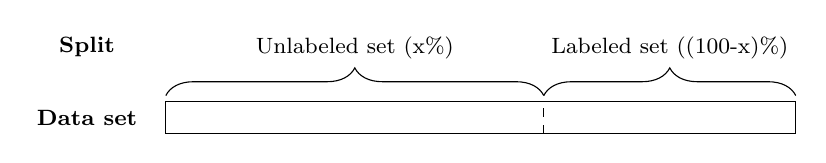
\begin{tikzpicture}[scale=0.8]
		\draw (0,0) rectangle (10,0.5) node[midway]{};
		\draw[dashed] (6,0) -- (6,0.5);
		
		\draw node[draw=none, xshift=-1cm, yshift=1.1cm, align=right] {\footnotesize \textbf{Split}};
		\draw node[draw=none, xshift=-1cm, yshift=.2cm] {\textbf{\footnotesize Data set}};
		
		\draw [decorate,decoration={brace,amplitude=10pt}, yshift=.1cm]
		(0,.5) -- (6,.5) node [black,midway,yshift=0.6cm] {\footnotesize Unlabeled set (x\%)};
		\draw [decorate,decoration={brace,amplitude=10pt}, yshift=.1cm]
		(6,.5) -- (10,.5) node [black,midway,yshift=0.6cm] {\footnotesize Labeled set ((100-x)\%)};
		\end{tikzpicture}
	\end{figure}
	
	\pause
	\begin{itemize}
		\item Data: Abalone, Digit, 20Newsgroup
		\item Default cross validation: 5 folds
		\item Similarity measure: Cosine for text, Euclidean similarity and Gaussian kernel for others
	\end{itemize}
	
	$\rightarrow$ Assume that we have pre-examined a fit graph construction method for our model.
\end{frame}

\begin{frame}
	\frametitle{Experimental Results (Thesis Page 29-31)}
	Results average in f1-score with split-x, (\#labeled, \#unlabeled)
	\begin{columns}
		\column{0.5\textwidth}
		\begin{table}
			\centering
			\captionsetup{justification=centering}
			\caption{Abalone data}
			\makebox[\textwidth][c]{
				\begin{tabular}{ cc }
					\textbf{Mincut} & \textbf{Graphical} \\
					\hline
					\multicolumn{2}{c}{Split-70, (1152:2690)} \\
					0.76 & 0.73 \\
					\hline
					\multicolumn{2}{c}{Split-97, (115:3727)} \\
					0.69 & 0.72 \\
					\hline
			\end{tabular}}
		\end{table}
		\column{0.5\textwidth}
		\begin{table}
			\centering
			\captionsetup{justification=centering}
			\caption{Digit data}
			\makebox[\textwidth][c]{
				\begin{tabular}{ cc }
					\textbf{Mincut} & \textbf{Graphical} \\
					\hline
					\multicolumn{2}{c}{Split-70, (539:1258)} \\
					0.99 & 0.99 \\
					\hline
					\multicolumn{2}{c}{Split-97, (53:1744)} \\
					0.95 & 0.95 \\
					\hline
			\end{tabular}}
		\end{table}
	\end{columns}
	
	\pause
	\vspace{-.5cm}
	
	\begin{table}
		\centering
		\captionsetup{justification=centering}
		\caption{comp vs rec, 20Newsgroups data}
		\makebox[\textwidth][c]{
			\begin{tabular}{ cc }
				\textbf{Mincut} & \textbf{Graphical} \\
				\hline
				\multicolumn{2}{c}{Split-70, (2661:6209)} \\
				0.85 & 0.85 \\
				\hline
				\multicolumn{2}{c}{Split-97, (266:8604)} \\
				0.41 & 0.84 \\
				\hline
		\end{tabular}}
	\end{table}
\end{frame}